\documentclass[11pt]{article}
\usepackage[utf8]{inputenc}
\usepackage{tikz}
\usepackage{amsmath,amsfonts,amsthm}
\usepackage[vlined, ruled]{algorithm2e}
\usepackage{geometry}
\usepackage[noend]{algpseudocode}
\usetikzlibrary{bayesnet}
\usepackage[nottoc,numbib]{tocbibind}
\setlength{\parskip}{1em}
\geometry{letterpaper,left=1.5in,right=1in,top=1in,bottom=1in}
\setlength\parindent{0pt}
\linespread{1.5}
\newcommand{\E}{\mathrm{E}}
\newcommand{\Var}{\mathrm{Var}}
\newcommand{\N}{\mathcal{N}}
\newcommand{\tr}{tr}

\begin{document}
\section{Introduction}
Human beings have an insatiable desire to understand, not only the things around us, but also ourselves. Why do we behave and respond the way we do \cite{hasson2012}? How do we learn and adapt \cite{hasson2004}\cite{hasson2005}? What do we believe or value \cite{Greene01}? These questions have mesmerized wise men for thousands of years, and the answers continue to evade us. For many of us, the key to all the secrets about ourselves is our brain, the central hub of all our thoughts and decision making. So, when a new technology emerged allowing us to study the brain in a quantitative manner, it opened countless doors of opportunities for those who possessed an aptitude for quantitative analysis and a hunger to learn more about our own identity.

Functional Magnetic Resonance Imaging, often referred to as fMRI, was first discovered and applied as a brain mapping method in 1990 by Seiji Ogawa \cite{Ogawa90}. Since then, this technology quickly popularized among Brain Science related research due to its unprecedented low health risk to subjects and its ability to accurately translate brain activities into highly-structured data \cite{Logothetis01}. Once the the highly abstract brain activities are converted into signs and digits, decoding patterns in the brain becomes a possibility. By treating each fMRI brain image as a feature vector, machine learning algorithms trained on a subset of the images may be used to distinguish cognitive information (e.g. which part of a movie someone is watching) from the held-out images \cite{Norman06}\cite{peterson12}\cite{peterson17}. These approaches typically treat each brain image in isolation, and attempt to identify patterns of activity associated with each of several candidate brain states. However, measurements from fMRI are often corrupted by noises created by the environment, human error, random neural activity, etc \cite{peterson11}. To address this issue, new branches of research has been emerging that specifically focuses on the extraction of useful information from noisy brain fMRI data by treating the brain images as a dynamic time series, and one of the most fruitful branches is functional connectivity \cite{peterson9} \cite{peterson19} \cite{peterson20}.

Functional connectivity analyses entail computing the correlations between the time series of activations each pair of brain regions exhibits. When we observe the brain, the neural activities can appear incredibly complex. But mechanics of brain are far from random: rather, the dynamic patterns of activity our brains exhibit are highly structured. Presumably this mirrors the complex but highly structured nature of our internal thoughts and experiences. Recently, it has become clear that important cognitive information is contained in higher-order brain patterns, such as the dynamic correlational structure of the data \cite{davidson2016}. When applying functional connectivity analyses on one subject in isolation, one can examine how (or whether) the correlational structure of these activity patterns (across a given set of brain regions) varies according to the cognitive task an experimental subject is performing \cite{Turke13}\cite{Rubinov2010}{peterson10}. Alternatively, the inter-subject functional correlation (ISFC) analyses applies functionally connectivity analyses across multiple subjects to isolate stimulus-dependent inter-regional correlations from intrinsic neural processes and non-neuronal noise \cite{hasson2016}\cite{jeremy2017}.

Over the past decade, functional connectivity analyses of brain data has evolved significantly \cite{olaf2005}\cite{khambhati2017}. However, there are three fundamental limitations to past approaches:

\begin{enumerate}
\item	\textbf{Correlation matrices are not scalable.} Examining pairwise correlation in brain data
produces a correlation matrix with O(n2) entries (where n is the number of brain regions). When n is large (e.g. the number of brain regions in an fMRI volume), the full correlation matrix can become unwieldy to compute with \cite{Rubinov2010}\cite{Betzel2017}\cite{Craddock2012}\cite{Yeo2011}. Furthermore, if one wishes to examine higher-order patterns (e.g. how correlations between correlations change over time), the storage requirements of the resulting patterns increase exponentially.

\item \textbf{The sliding window approach is not well suited to studying dynamic activity.} Most approaches to calculating functional connectivity uses the sliding window method, where a window of set time length is selected to calculate the functional connectivity at one time point before the window is shift forward for following calculations \cite{enrico2011}\cite{elena2012}. One disadvantage of the sliding window approach is the loss of information for a number of time points equal to the sliding window length. Although many practical applications use buffers to make up for the loss, repeated application of the sliding window approach on the same dataset—--e.g. calculating the correlation of the correlation between nodes—--is impractical. In addition, the sliding window approach provides only a poor approximation of the moment-by-moment patterns at the heart of these representations.

\item \textbf{Only using node activations and first level dynamic patterns may not be enough.} The brain is a network of seemingly autonomous nodes that are actually intricately interconnected. Useful information about the brain may exist within interactions between interactions between nodes (2nd order), interactions between interactions between interactions (3rd order), or in even higher order dynamics. To fully grasp the functions of a single node in the network, it is crucial to understand of its activities relative to the richly woven network that supports it. Therefore, incorporating information from higher order dynamics could potentially improve the quality of brain analysis.

\end{enumerate}

Here, we present the High-Order Brain Dynamics (HOBD), a model that seeks to understand the dynamics behind different "levels" of interaction between brain structures and how this information is represented in the brain. To efficiently access and analyze brain dynamics at higher levels, the HOBD model revolutionizes functional connectivity calculation methods and creates a means to repeatedly "level up" brain dynamics information, computing higher level functional connectivity from low level information. These changes have notably improved the recovery accuracy of brain correlation structures, and significantly increased decoding capabilities using a limited amount brain data.

First, to find an effective replacement for the widely used sliding window method, we designed TimeCorr, an intuitive method that found inspiration directly from the fundamental correlation function. Like the sliding window method, TimeCorr is able is able to recover functional connectivity from fMRI brain images with similar if not higher accuracy. But TimeCorr goes beyond the sliding window method by (a) not requiring buffer at each end for calculation, thereby avoiding data loss, (b) offering extra stability by using all the time points in the time series for calculation of correlation at every time point, (c) provides the option to shift between locality and fluidity based on user demand by varying the resolution parameter.

TimeCorr achieves all the above functions through the use of Gaussian distribution. By attaching a Gaussian coefficient to each time point component in the time series, TimeCorr is able to allocate the amount of influence each neighboring time point has on the calculation of correlation at the time point of interest. As the Gaussian center (highest density/coefficient) is always at the time point of interest, TimeCorr guarantees to return highly accurate approximations of the temporal ground truth. In addition, the user can choose to have more fluidity in overall results by choosing coefficients from a Gaussian distribution with a large variance; or higher resolution and more locality by choosing coefficients from a distribution with a smaller variance.

Second, we designed a "level up" method that applies TimeCorr, Inter-Subject Functional Connectivity (ISFC) and Principle Component Analysis (PCA) to calculate higher order functional connectivity. To overcome the problem of scaling and to enforce uniformity for inter-levels analysis, we use TimeCorr on each subject to calculate functional connectivity from previous level activations and then reduce the results to an arbitrary number of feature points to represent the activations for the next level. As TimeCorr avoids data loss in calculating functional connectivity and PCA maintains an uniform number of activations at each "level up", we are able to obtain $10^{th}$ order functional connectivity while ensuring linear scaling in storage and computation.

We believe that different orders of functional connectivity represents information on different aspects of brain dynamics, and incorporating knowledge of the higher-order structures of the brain will expand present brain decoding capabilities. To measure the amount of information present at each level, we introduce decoding accuracy, a testing parameter that describes the proportion of time points in one level of a subject's functional connectivity graph that has the highest correlation with the same time point from the average activations of all other subjects. We are interested in how decoding accuracy changes as we reach higher order functional connectivity. Although we presumed brain dynamics would converge as we get to higher orders and decoding accuracy would increase, reality proved otherwise. This is shown and discussed in more detail in the Intra-Level Decoding Analysis section of our results.

To carry out an in-depth evaluation of the effectiveness of the HOBD model, we also conducted the Multi-Level Mixture Analysis. This study aims to understand how the dynamic information of different levels of interactions between brain regions can be used to improve brain pattern decoding capabilities. In the Multi-Level Mixture Analysis section of our results, we provide a side by side comparison that highlights the improvements achieved by a mixture model that incorporates multiple levels of functional connectivity. In the process of finding the mixture model that maximizes decoding accuracy, we also explored the utility of each level of brain dynamics through analysis of the distribution of optimal level weights. The methods and findings will be discussed extensively in the results section.

\section{Model Description}
The High-Order Brain Dynamics model seeks a new perspective to understanding the dynamics behind stimulus-driven brain activities. Utilizing the capabilities and advantages of TimeCorr and "Level Up", the HOBD model attempts to incorporate information on high-order brain dynamics into its analysis of the brain.

\subsection{Single Subject TimeCorr}
The TimeCorr method was designed for the purpose of replacing the sliding window method as a lossless alternative to achieve more accurate calculation of functional connectivity (the correlation structure between brain regions within a subject's brain) from brain fMRI data. The sliding window method operates by applying the correlation calculation function on a block of data centering on the time point of interest $t$ and spanning $L_w$ time points, where $L_w$ is the sliding window length and must be of considerable magnitude for the sliding window method to achieve respectable accuracy. However, due to its inherent design flaw, using the sliding window method on a dataset of time length $T$ could only yield functional connectivity for $T-L_w$ data points, a loss not insignificant due to the typical magnitude of $L_w$. Thus, as calculating high order functional connectivity involves repeatedly applying the method of correlation calculation on the dataset, using the sliding window method would result in rapid deterioration in the amount of usable data. In addition, as the sliding window method uses a long block of data for correlation calculation, it can only achieve a rough approximation of the general average in the block and not the instantaneous truth at each time point.

To solve these problems, we designed the TimeCorr method, which finds inspiration from the fundamental correlation function. Instead of isolating a block of points for correlation calculation, TimeCorr effectively utilizes information from the entire dataset for functional connectivity calculation at every time point. To ensure locality of TimeCorr's results, every term is multiplied by a weight drawn from a normalized Gaussian density function so that each time point influences the calculation of functional connectivity at time point of interest $t$ proportional to its distance from $t$. This adaptation of the correlation function effectively eliminates results repetition at the beginning and end of the time series, thereby increasing the number of output time points to equal to the number of inputs and avoiding any data loss. In addition, through the application of Gaussian density coefficients, TimeCorr gives more significance to information closer to the time point of interest in its calculations, thereby ensuring a more accurate estimation of instantaneous correlation.

\large{\textbf{Formal Definition}}

\normalsize
Given a single subject fMRI dataset with T time points and N brain regions, to apply TimeCorr:

\begin{enumerate}
\item Base on the amount of influence neighboring time points should have on the calculation of the functional connectivity at each time point, choose variance V for the Gaussian density function to generate coefficients.

\item For each time point t:
\begin{enumerate}
\item Using a Gaussian density function of variance V and mean $t$, generate an array of coefficients $w_t$ of length T.

\item For each brain region, element-wise multiply its activation time sequence $a_i$ by the coefficients array to create a weighted activations array $S^i_t$.

\item Find the temporal correlation between brain region i and brain region j at time point t through the equation:

\begin{align*}
C(S^i_t,S^j_t) = \frac{1}{Z}\frac{\sum_{l=0}^T (S_l^i - \bar{S^i_t})\cdot(S^j_l - \bar{S^j_t})\cdot \mathcal{N}(l|t,\sigma)}{\sigma_{S_t^i} \cdot \sigma_{S_t^j}}
\end{align*}
Where
\begin{align*}
Z &= \sum_{l=0}^T \mathcal{N}(l|t,\sigma)\\
\bar{S^i_t} &=\frac{1}{Z} \sum_{l=0}^T S^i_l \cdot \mathcal{N}(l|t,\sigma)\\
\sigma_{S_t^i} &=\sqrt{ \frac{1}{Z}\sum_{l=0}^T (S_l^i-\bar{S_t^i})^2 \cdot \mathcal{N}(l|t,\sigma)}\\
\end{align*}
\item Repeat above process for every pair of brain regions to create correlation matrix for time point t
\item Convert the correlation matrix at every time point to its inverse squareform format, output an array of size $T$ by $(V^2-V)/2$ dimensional matrix, where $T$ and $V$ represent the time length and brain region count of the dataset.
\end{enumerate}
\end{enumerate}

The addition of the Gaussian density variance parameter V gives the user the extra freedom to customize the desired level of resolution for correlation calculation. If a large variance is chosen, the influence of neighboring time points on the calculation of functional connectivity at each time point is increased, thereby adding smoothness and stability to the resulting functional connectivity time sequence and providing a more accurate representation of the general trend. But if a small variance is chose, most of the weight will be placed on the time point of interest and its immediate neighbors, and so the resulting functional connectivity time sequence will have more emphasis on local accuracy. After experimenting with different setups, we discovered that the best way to distribute weights for time points in the time series is to apply a Gaussian probability density function centered around the time point of interest with variance equal to the minimum between the total number of time points and 1000. This finding will be discussed in more detail in the Results section.

In contrast to the sliding window method, which is widely considered to be the golden standard for fMRI functional connectivity calculation, the TimeCorr approach is able to more accurately retrieve the temporal correlation at each time point without loss of important data. This advantage makes it possible to "level up" to higher order functional connectivities---progressively finding the correlation of correlations---and explore dynamics and patterns heretofore untouched. We will go into more detail about the "level up" process and high order functional connectivity in the "Leveling Up" section.

\subsection{Inter-Subject Functional Correlations using TimeCorr}

The Inter-Subject Functional Correlations (ISFC) is a process of calculating functional connectivity between brain regions of different subjects \cite{jeremy2017}\cite{hasson2016}. The patterns recovered by ISFC is analogous to single subject functional connectivity (which reflect the correlational structure across brain regions within an individual's
brain), but they should reflect only activity that is specifically stimulus-driven. For every subject, we compare its brain activations time sequence $a_i$ with the average activations of all other subjects $a_{-i}$. Through the process of averaging activations of multiple subject, we dampen the effect of noise and enhance stimulus-dependent activations in $a_{-i}$. Therefore, when we calculate the functional connectivity matrix between subject activation $a_i$ and the average response from the rest of the participants $a_{-i}$, the functional connectivity we calculate are more likely to reflect activities that are stimulus-driven.

Furthermore, after we obtain the functional connectivity matrix between each subject and the average of their counterparts, we use Fisher Z-transformation to average the results from all the subjects. In addition to the noise-dampening and stimulus-enhancing effects that comes with averaging, we are also able to gain an unbiased view of the overall connectivity pattern across all subjects within our analysis. Fisher Z-transformation is applied in the averaging process as a means to stabilize and reduce approximation variance to return a less biased result than from directly averaging correlations.

\large{\textbf{Formal Definition}}

\normalsize
Given a fMRI dataset of $S$ subjects, each with T time points and N brain regions, to apply TimeCorr ISFC:
\begin{enumerate}
\item Determine the desired temporal resolution for calculation and select $\sigma$, the Gaussian density function variance for TimeCorr coefficients generation.
\item For each subject s,
\begin{enumerate}
\item Find the average activation of all other subjects:
\begin{align*}
O_s=\frac{\sum_{i\neq s}^N S_i}{N-1}
\end{align*}
where $S_i$ represents the activation matrix for subject $i$ and $N$ represents the total number of subjects.
\item Find the functional connectivity between the brain activations $S$ for subject $s$ and the average brain activations of all other subjects $O$ using TimeCorr ISFC with variance $\sigma$. The correlation between $S^i_t$---activation of brain region i for subject $s$ at time $t$---and $O^j_t$---average brain activation of brain region $j$ of other subjects at time points $t$---is obtained through the following equation:
\begin{align*}
C(S^i_t,O^j_t) = \frac{1}{Z}\frac{\sum_{l=0}^T (S_l^i - \bar{S^i_t})\cdot(O^j_l - \bar{O^j_t})\cdot \mathcal{N}(l|t,\sigma)}{\sigma_{S_t^i} \cdot \sigma_{O_t^j}}
\end{align*}
Where
\begin{align*}
Z &= \sum_{l=0}^T \mathcal{N}(l|t,\sigma)\\
\bar{S^i_t} &=\frac{1}{Z} \sum_{l=0}^T S^i_l \cdot \mathcal{N}(l|t,\sigma)\\
\bar{O^i_t} &=\frac{1}{Z} \sum_{l=0}^T O^i_l \cdot \mathcal{N}(l|t,\sigma)\\
\sigma_{S_t^i} &=\sqrt{ \frac{1}{Z}\sum_{l=0}^T (S_l^i-\bar{S_t^i})^2 \cdot \mathcal{N}(l|t,\sigma)}\\
\sigma_{O_t^i} &=\sqrt{ \frac{1}{Z}\sum_{l=0}^T (O_l^i-\bar{O_t^i})^2 \cdot \mathcal{N}(l|t,\sigma)}\\
\end{align*}
\item Repeat the above process for every pair of brain regions, for every time point.
\end{enumerate}
\item Apply Fisher Z-transformation to every element $r$ of the correlation matrices for each subject at each time points to obtain the corresponding Z-correlation matrices:
\begin{align*}
z = \frac{1}{2}\ln(\frac{1+r}{1-r})
\end{align*}
\item Average the Z-correlation matrices $Z_i$ across all subjects:
\begin{align*}
S_Z = \frac{1}{N}\sum^N_{i=1}Z_i
\end{align*}
\item Apply inverse Z-transformation to the average Z-correlation matrix to obtain the Inter-subject Functional Connectivity (ISFC) mean correlation matrix:
\begin{align*}
ISFC = \frac{\exp(S_Z+S_Z^T)-1}{\exp(S_Z+S_Z^T)+1}
\end{align*}
\item Convert the correlation matrix at every time point to its inverse squareform format, and output a $T$ by $(V^2-V)/2$ dimensional matrix containing the average functional connectivity of all subjects in the dataset, where $T$ and $V$ represent the time length and brain regions count of the dataset, respectively.
\end{enumerate}

\subsection{Multi-Subject TimeCorr Level-Up}
The multi-subject TimeCorr Level-Up process utilizes the functionalities of the single-subject TimeCorr method to extract high-order brain dynamics patterns from brain fMRI data. Due to the data-losing flaw of the sliding window method, research related to functional connectivity heretofore have been largely limited to analysis on raw fMRI activations and first level functional connectivity. However, with the availability of TimeCorr, we are able to repeatedly find higher order functional connectivity of an fMRI dataset without fear of losing data with each "level up". This advantage allows us to explore higher-order dynamic patterns within the brain that was previously impossible to access.

The concept of "leveling up" involves repeatedly finding the correlation of correlations of brain activity. Given a brain fRMI dataset, we designate the raw activations as level 0 and the functional connectivity (correlation structure) of the activations as level 1, the result of "leveling up" from level 0 (here "level" and "order" are interchangeable). Hereafter, given a matrix of functional connectivity of level $n$, we can apply the TimeCorr Level-Up method to find the correlation structure of the data at level $n$ to obtain functional connectivity at level $n+1$.

In addition to effectively retaining all relevant data, the Multi-Subject TimeCorr Level-Up method also presents a scalable solution to large datasets. Normally, for an input dataset of $V$ voxels (brain regions), the first order functional connectivity would occupy $V^2$ space and every additional level of functional connectivity would involve an exponential increase in storage requirement. In order to circumvent this problem, the Multi-Subject TimeCorr Level-Up method first finds the inverse square-form (vectorized array containing the non-diagonal elements of a square matrix) of the correlation matrices for every time point in the "level up" output, and then uses PCA to further reduce the result to a matrix of $T$ by $V$ dimensions, where $T$ and $V$ represent the time length and voxel count of the input dataset. This solution ensures all orders of functional connectivity derived from the same dataset will have the same dimensions. In addition, the application of PCA further guarantees that only the most principle components of each functional connectivity matrix is retained for further analysis.

\large{\textbf{Formal Definition}}

\normalsize
Given a brain activation or activation correlation matrix at level $l$ of dimensions S subject, V brain regions and T time points, the Level-Up function

\begin{enumerate}
\item Applies single-subject TimeCorr on the data matrix for each subject to obtain correlations matrix

\item Concatenate the correlations matrix for each subject from the previous step together along the first dimension into a single matrix of dimensions $(S*V)xT$

\item Apply PCA on the concatenated matrix from the previous step to obtain a reduced representation of the correlation matrix

\item Separate the reduced correlation matrix from the previous step into data for each subject to obtain a 3-D matrix of size SxVxT

\item Repeat the above process on the output to level up again

\end{enumerate}

\subsection{Multi-Subject Decoding Analysis with TimeCorr ISFC}
The Multi-Subject Decoding Analysis is a method designed to find stimulus-dependent activations in fMRI dataset by cross referencing data from multiple subjects \cite{jeremy2017}. Through application of Multi-Subject TimeCorr ISFC on two equal divisions of the subject data, "white noises" (background noise, human error, random neural activity, etc) are dampened and activities that are common across subjects are emphasized, thereby increasing the salience of patterns that reflect activities that are only stimulus-driven. Additionally, when the correlation between the same time point in both sub-groups is high, it indicates that the average brain activities in one group demonstrates very high similarity with the average brain activities of all subjects in the other group at that time point. When the brain activities of multiple subjects display high similarity for certain time points in their brain activations time sequence, then intuitively there's a high probability that their brain responses for those time points are uniformly caused by their common stimulus. Using this logic, the decoding accuracy of the dataset, percentage of time points that demonstrates highest correlation with themselves across two sub-division of subject data, gives an accurate representation of

\begin{enumerate}
\item Similarity between subject responses throughout the fMRI simulation
\item The average proportion of subject activities within the dataset that are stimulus dependent
\item The average proportion of subject activities that shows significant distinction from the rest of the time sequence
\item The potency of stimuli in generating salient cognitive response across all subjects
\end{enumerate}

Due to the above characteristics, the Decoding Analysis makes up a crucial part of our project as a means to evaluate the effectiveness of our newly developed methods.

\large{\textbf{Formal Definition}}

\normalsize
Given a multi-subject dataset containing $S$ subjects, each possessing $T$ time points and $V$ voxels, to conduct Decoding Analysis:
\begin{enumerate}
\item Select a Gaussian density variance V for TimeCorr coefficient generation.
\item For n repetitions:
\begin{enumerate}
\item Randomly divide the subjects into two equal groups.
\item Calculate Inter-Subject Functional Connectivity (ISFC) for each group using TimeCorr. The resulting ISFC matrices are labelled $I_1$ and $I_2$.
\item Calculate time-point-wise correlation between functional connectivity at each time point in $I_1$ and functional connectivity at each time point in $I_2$, resulting in a $T$ by $T$ correlation matrix.
\item A time point in $I_1$ is correctly decoded if the time point of highest correlation in $I_2$ is the same time point, and vice versa for $I_2$.
\item Count and record the number of time points that were correctly decoded for $I_1$ and $I_2$.
\end{enumerate}
\item Sum the total number of time points correctly decoded for $I_1$ and $I_2$ across all repetitions, and find the average through dividing by the product between the repetition count and two times the time point count (to account for both $I_1$ and $I_2$). The result is the decoding accuracy output of the multi-subject dataset.
\end{enumerate}

\section{Results}
\subsection{Testing Single Subject TimeCorr on Synthetic Datasets}
To conduct a side-by-side comparison of the correlation recovery functionalities between the TimeCorr method and the traditional sliding window method, we constructed synthetic datasets with pre-defined correlation patterns using Cholesky decomposition. This approach takes an original X variable (or matrix) and uses the Cholesky transformation to create a new, correlated, Y variable. Using this approach, we are able generate a time sequence of synthetic brain activations that exactly follows a pre-designated a dynamically correlation structure.

Two kinds of synthetic datasets were generated to test different features of TimeCorr:
\begin{enumerate}
\item Single Subject Synthetic Dataset with block correlations

In this dataset, we divide time sequence into $N$ blocks of equal time lengths. Each block possesses a different correlation that's consistent throughout the length of the block. This dataset will be used to test TimeCorr's ability to distinguish different correlations within a dataset. To generate the dataset:
\begin{enumerate}
\item Using random normal distribution, generate a dataset X of dimensions $T$ by $V$, where $T$ and $V$ represents the desired time length and voxel (brain region) count, respectively.
\item Design a correlation matrix of dimensions $V$ by $V$ for each of the $N$ blocks, denoted $R_n$.
\item For each of the $N$ blocks in X, transform the block $X_n$ into correlated structure through the equation:
\begin{align*}
W_n = Cholesky(R_n) \cdot X_n
\end{align*}
Where $Cholesky(R_n)$ represents the Cholesky decomposition of the correlation matrix $R_n$
\item Piecing all of the blocks together to form the new synthetic dataset W that possesses the designated dynamic correlation structure.
\end{enumerate}

\begin{figure}[ht]
\caption{Testing on 10 blocks of different correlations}
\includegraphics[width=1\textwidth]{../figures/SyntheticTesting/10block100tCopy.png}
\label{fig:10block100t}
(a) In the first row, solid lines show the correlation between block correlations and TimeCorr solutions; dotted, sliding window solutions. (b) In the second row, solid lines show mean squared error(MSE) between block correlations and TimeCorr solutions; dotted, sliding window solutions. (c) In the third row, the solid line shows correlation between temporal ground truth and TimeCorr solutions; dotted, sliding window solutions. (d) In the fourth row, the solid line shows MSE between temporal ground truth and TimeCorr solutions; dotted line, sliding window solutions. (e) The columns represent TimeCorr implementations with a different Gaussian density variances.
\end{figure}

The average results of running TimeCorr and the sliding window method on 100 datasets containing 10 blocks, each occupying 100 time points, is displayed in Figure \ref{fig:10block100t}. In the graphs on the first row, each color represents the correlation between the correlation structure of a block with the solutions from the TimeCorr and the sliding window approach, which are represented by solid and dotted lines, respectively. The graphs show that both the TimeCorr and the sliding window approach are able to effectively recover the correct correlation structure for each block. In addition, the TimeCorr approach is able to more accurately recover the temporal block correlation at each time point when the Gaussian density variance for its coefficient generation is low (in other words, when the resolution is high). In contrast, when the TimeCorr Gaussian variance increases, the solutions slowly gains smoother transition in-between correlation blocks but in exchage for lower recovery resolution and lower temporal accuracy.

These results are confirmed by the results shown in the second row, which shows the MSE between the block correlations and the TimeCorr and the sliding window solutions, which are represented by solid and dotted lines, respectively. TimeCorr and the sliding window approach seem to have very similar performances when the TimeCorr variance is low. But as the Guassian density variance for TimeCorr coefficients generation increases, the mean squared error of TimeCorr decreases significantly, indicating that TimeCorr is able to produce more precise solutions at block centers when the Gaussian density variance is high.

The graphs in the third and fourth row show the correlation and MSE between the temporal ground truth (true correlation at each time point) and the TimeCorr and the sliding window solutions, represented by solid and dotted lines respectively. As the Gaussian variance of TimeCorr increases, the correlation between its solution and the ground truth at transitions improves drastically, and the mean squared error experiences significant improvements across the board. When comparing the TimeCorr results with the sliding window results in these two rows, we can see that TimeCorr performs significantly better in both correlation and MSE when the TimeCorr variance is high.

\begin{figure}[ht]
\caption{Testing on 2 blocks of different correlations}
\includegraphics[width=1\textwidth]{../figures/SyntheticTesting/2block250t.png}
\label{fig:2block250t}
(a) In the first row, solid lines show the correlation between block correlations and TimeCorr solutions; dotted, sliding window solutions; dot-dashed, ground truth. (b) In the second row, solid lines show mean squared error(MSE) between block correlations and TimeCorr solutions; dotted, sliding window solutions; dot-dashed, ground truth. (c) In the third row, the solid line shows correlation between temporal ground truth and TimeCorr solutions; dotted, sliding window solutions; gray, random guess. (d) In the fourth row, the solid line shows MSE between temporal ground truth and TimeCorr solutions; dotted line, sliding window solutions; gray, random guess. (e) The columns represent TimeCorr implementations with a different Gaussian density variances.
\end{figure}

To further confirm our results, we rerun the test on 100 dataset containing 2 blocks of different correlations, each containing 250 time points. The average results are shown in Figure \ref{fig:2block250t}, with ground truth and random guess displayed for comparison. From these graphs, we can can confirm TimeCorr boasts significantly better performances than the sliding window approach in both correlation and MSE when the ground truth correlation is stable. Furthermore, TimeCorr is able to more effectively recover correlations structures at abrupt transitions using a high resolution setup (low Gaussian variance).

\item Single Subject Synthetic Dataset with ramping correlations

In this dataset, we adopt a correlation structure that linearly changes from one correlation $C_1$ to another correlation $C_2$. This dataset will be used to test TimeCorr's ability to accurately recover correlation structures that are dynamically changing over time.

\begin{enumerate}
\item Using random normal distribution, generate a dataset X of dimensions $T$ by $V$, where $T$ and $V$ represents the desired time length and voxel (brain region) count, respectively.
\item Generate two correlation matrices $C_1$ and $C_2$, then generate temporal correlation structures $C_t = z2r(\frac{(T-t) \cdot r2z(C_1)}{T} + \frac{t\cdot r2z(C_2)}{T})$, where T is the total time length of the dataset and r2z and z2r is Fisher Z-transformation and inverse Fisher Z-transformation, respectively, to ensure stable combination of correlation structures.
\item For activations $X_t$ at each time point in X, transform the data into correlated structure through the process:
\begin{align*}
W_t = Cholesky(C_t) \cdot X_t
\end{align*}
\item Piecing all of the blocks together to form the new synthetic dataset W that possesses the designated dynamic correlation structure.
\end{enumerate}
\end{enumerate}

\begin{figure}[ht]
\caption{Testing on 1000 time point ramping dataset}
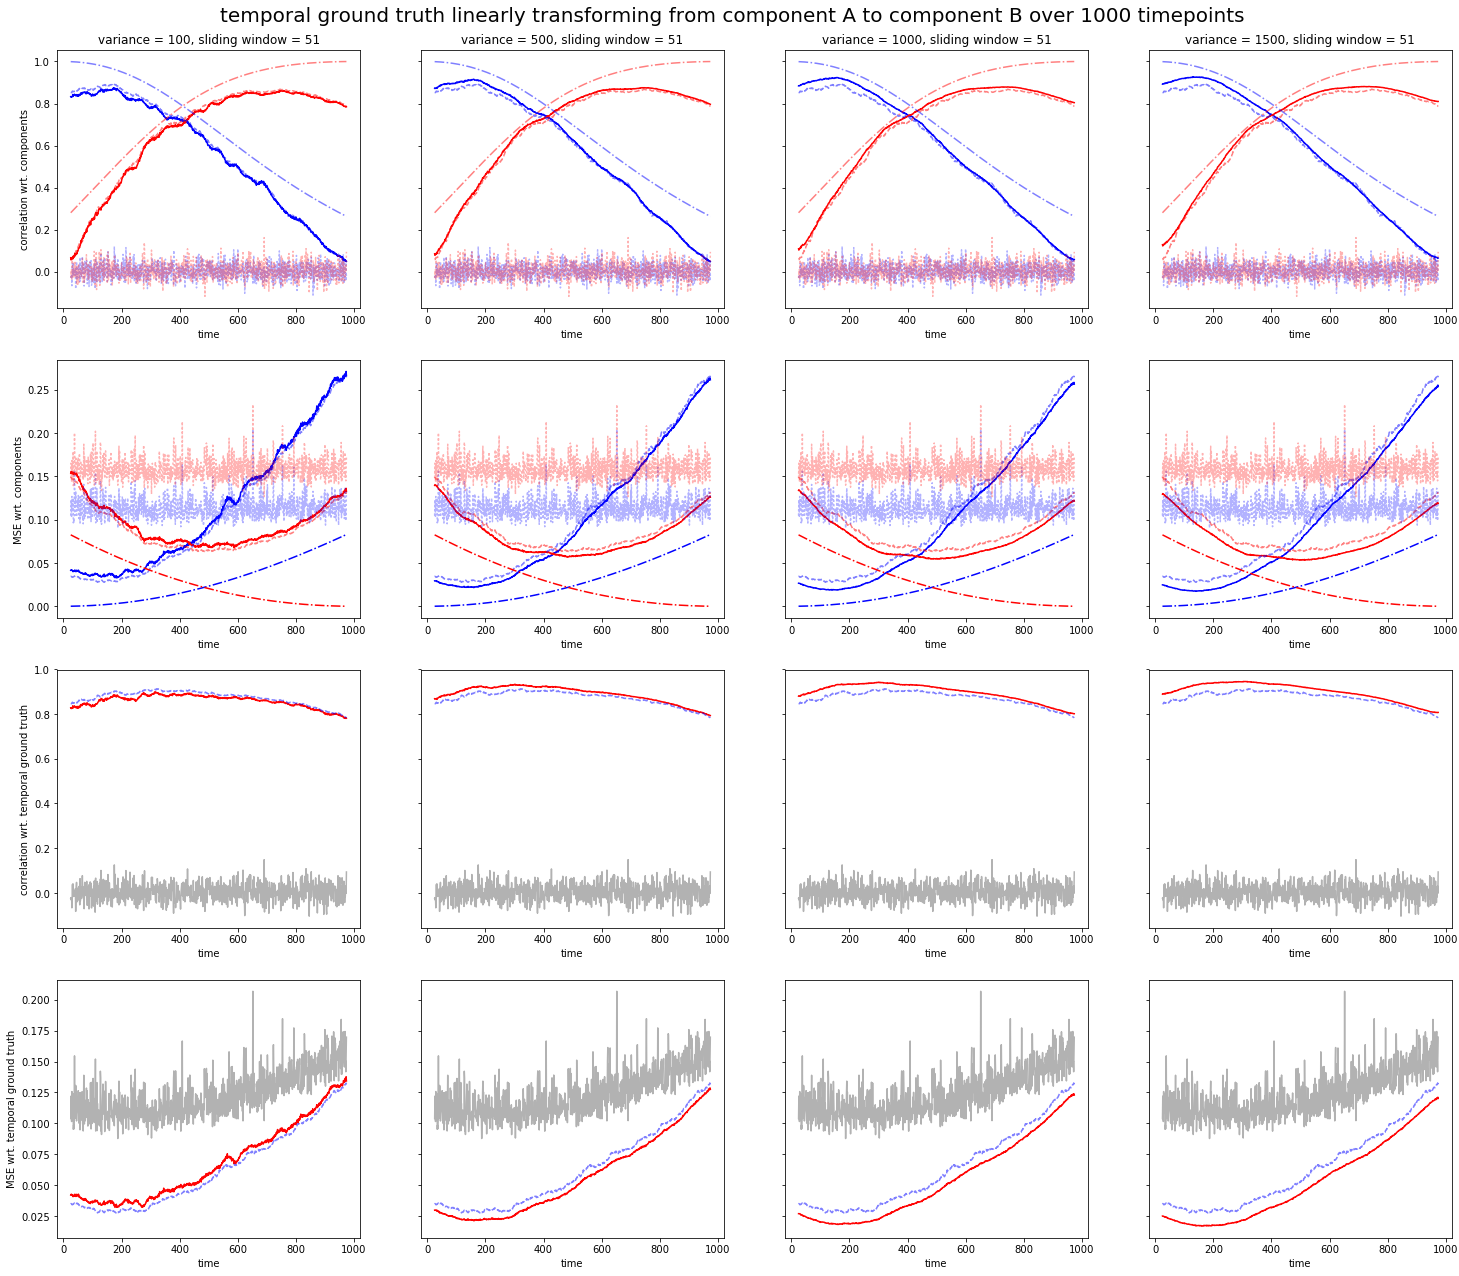
\includegraphics[width=1\textwidth]{../figures/SyntheticTesting/ramp1000t4var.png}
\label{fig:ramp1000t4var}
(a) In the first row, solid lines show the correlation between block correlations and TimeCorr solutions; dotted, sliding window solutions; dot-dashed, ground truth. (b) In the second row, solid lines show mean squared error(MSE) between block correlations and TimeCorr solutions; dotted, sliding window solutions; dot-dashed, ground truth. (c) In the third row, the solid line shows correlation between temporal ground truth and TimeCorr solutions; dotted, sliding window solutions; gray, random guess. (d) In the fourth row, the solid line shows MSE between temporal ground truth and TimeCorr solutions; dotted line, sliding window solutions; gray, random guess. (e) The columns represent TimeCorr implementations with a different Gaussian density variances. (f) In the first two rows, the blue lines represent the relationship between recovered solution and the left terminal correlation; red line, right terminal correlation.
\end{figure}

First, 100 ramping datasets with 1000 time points were generated to produce a gradual linear transition between two distinct correlation structures. The average results are displayed in Figure \ref{fig:ramp1000t4var}. At Gaussian variance equal to 100, TimeCorr shows very similar performance with the sliding window method with a window length of 51, albeit TimeCorr results do not come at the expense of extensive data-loss. When the Gaussian variance of TimeCorr is increased to above 100, the TimeCorr solutions' advantages over the sliding window solution immediately becomes obvious in both MSE and their correlation with the temporal ground truths. This phenomenon is most evident in the third and fourth row, where the TimeCorr solutions consistently shows higher correlation and lower MSE with the ground truth at almost every time point.

\begin{figure}[ht]
\caption{Testing on 500 time point ramping dataset}
\includegraphics[width=1\textwidth]{../figures/SyntheticTesting/ramp500t4var.png}
\label{fig:ramp500t4var}
(a) In the first row, solid lines show the correlation between block correlations and TimeCorr solutions; dotted, sliding window solutions; dot-dashed, ground truth. (b) In the second row, solid lines show mean squared error(MSE) between block correlations and TimeCorr solutions; dotted, sliding window solutions; dot-dashed, ground truth. (c) In the third row, the solid line shows correlation between temporal ground truth and TimeCorr solutions; dotted, sliding window solutions; gray, random guess. (d) In the fourth row, the solid line shows MSE between temporal ground truth and TimeCorr solutions; dotted line, sliding window solutions; gray, random guess. (e) The columns represent TimeCorr implementations with a different Gaussian density variances. (f) In the first two rows, the blue lines represent the relationship between recovered solution and the left terminal correlation; red line, right terminal correlation.
\end{figure}

TimeCorr's performance advantage is further verified by the testing results from 100 ramping datasets of 500 time points, where the linear transitions between the two distinct terminal correlation structures are accelerated from the 1000 time point datasets. The average results are shown in Figure \ref{fig:ramp500t4var}. In contrast to the results from the 1000 time point datasets, the performance difference is more evident in the results from the 500 time point datasets. As the temporal ground truth correlation linearly transitions from the left terminal correlation structure to the right terminal correlation structure within 500 time points, the rate of change at each time point is much greater than that of the 1000 time point dataset. Under these conditions, the TimeCorr results consistently shows significantly higher correlation and lower MSE with the temporal ground truths than the sliding window results. This result indicates that the TimeCorr approach is better at recovering rapidly changing dynamic correlation structures than the sliding window approach. In addition, the results does not seem to change significantly from the 500 variance TimeCorr implementation to the 1500 variance TimeCorr implementation, which might be due to the variance exceeding the dataset time length.

\begin{figure}[ht]
\caption{Testing on 100 time point ramping dataset}
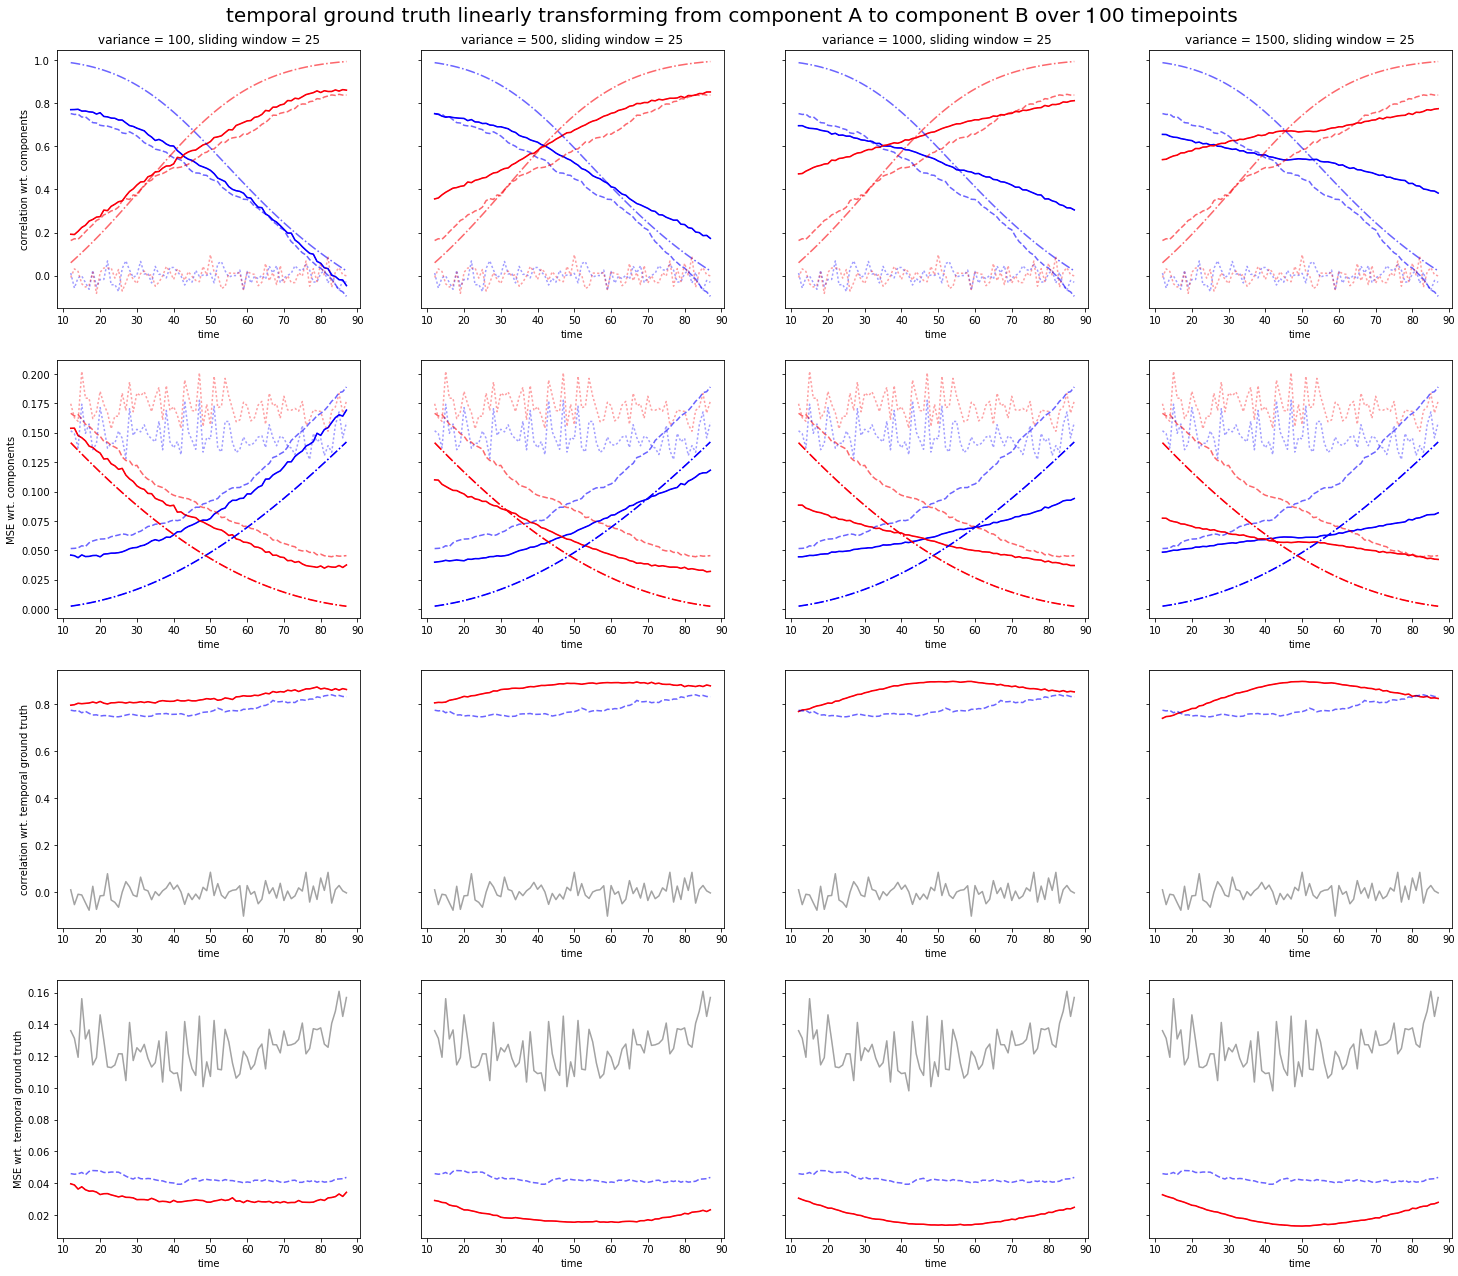
\includegraphics[width=1\textwidth]{../figures/SyntheticTesting/ramp100t4var.png}
\label{fig:ramp100t4var}
(a) In the first row, solid lines show the correlation between block correlations and TimeCorr solutions; dotted, sliding window solutions; dot-dashed, ground truth. (b) In the second row, solid lines show mean squared error(MSE) between block correlations and TimeCorr solutions; dotted, sliding window solutions; dot-dashed, ground truth. (c) In the third row, the solid line shows correlation between temporal ground truth and TimeCorr solutions; dotted, sliding window solutions; gray, random guess. (d) In the fourth row, the solid line shows MSE between temporal ground truth and TimeCorr solutions; dotted line, sliding window solutions; gray, random guess. (e) The columns represent TimeCorr implementations with a different Gaussian density variances. (f) In the first two rows, the blue lines represent the relationship between recovered solution and the left terminal correlation; red line, right terminal correlation.
\end{figure}

To further verify the advantages of TimeCorr in recovering highly dynamic correlation structures and the limitations of changing TimeCorr Gaussian variance in datasets with short time lengths, we conducted analysis on 100 ramping datasets of only 100 time points, where the linear transitions between the two distinct terminal correlation structures are further accelerated from the 500 time point datasets. The results are shown in Figure \ref{fig:ramp100t4var} and confirm our observations from the previous tests: the TimeCorr approach consistently out-performs the sliding window approach in every setup and TimeCorr's performance stagnates/worsens as its Gaussian variance increases beyond the total time length of the dataset. These results further consolidates TimeCorr's superiority over the sliding window method in recovering highly dynamic correlation structures. In addition, we gained very useful insight on how to select Gaussian variance for TimeCorr to produce the best recovery results.

\begin{figure}[ht]
\caption{Testing on 100 time point ramping dataset}
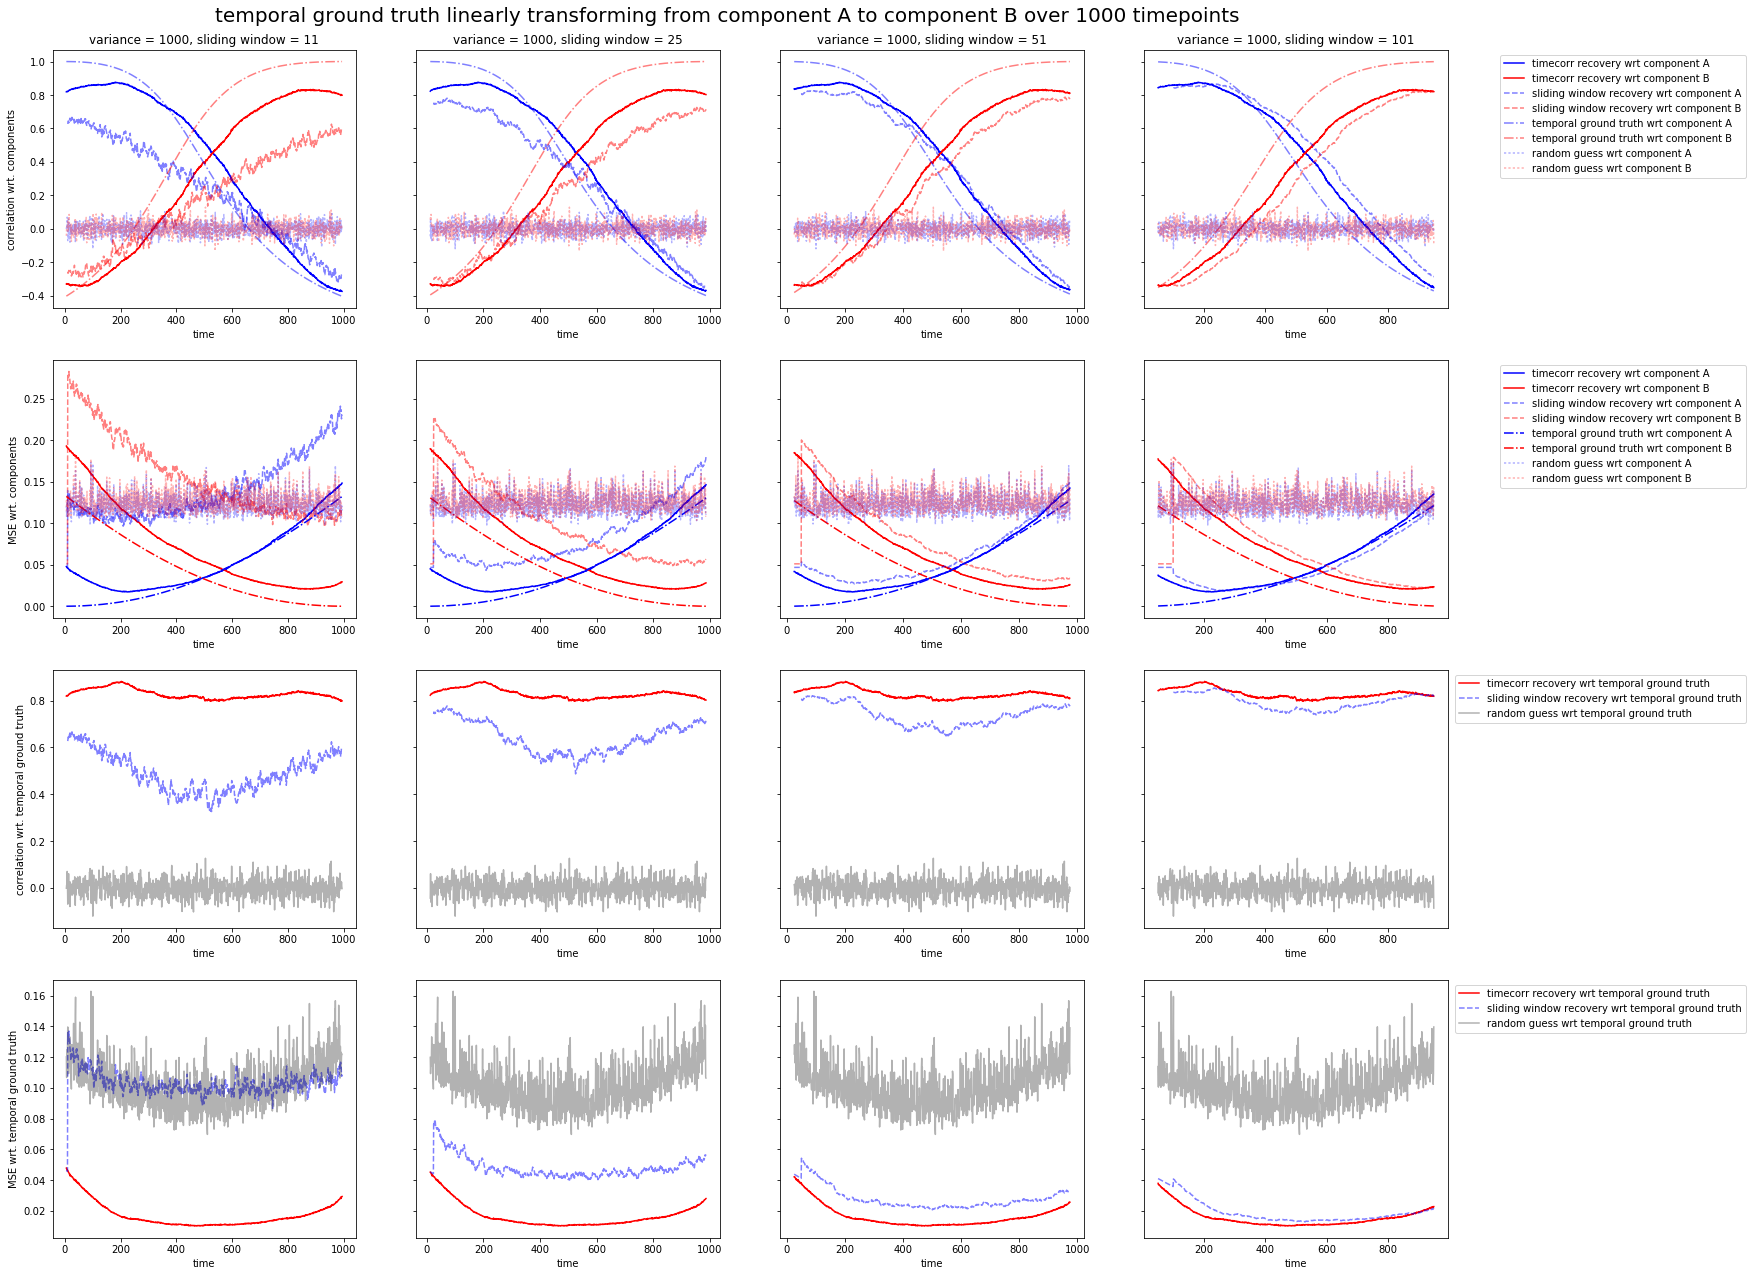
\includegraphics[width=1\textwidth]{../figures/SyntheticTesting/ramp1000t4slide.png}
\label{fig:ramp1000t4slide}
(a) In the first row, solid lines show the correlation between block correlations and TimeCorr solutions; dotted, sliding window solutions; dot-dashed, ground truth. (b) In the second row, solid lines show mean squared error(MSE) between block correlations and TimeCorr solutions; dotted, sliding window solutions; dot-dashed, ground truth. (c) In the third row, the solid line shows correlation between temporal ground truth and TimeCorr solutions; dotted, sliding window solutions; gray, random guess. (d) In the fourth row, the solid line shows MSE between temporal ground truth and TimeCorr solutions; dotted line, sliding window solutions; gray, random guess. (e) The columns represent different sliding window implementations with varying window lengths. (f) In the first two rows, the blue lines represent the relationship between recovered solution and the left terminal correlation; red line, right terminal correlation.
\end{figure}

Lastly, to demonstrate TimeCorr's advantage over the sliding window approach generalizes to all setups, we conducted an analysis on 100 ramping datasets, each containing 1000 time points, to compare TimeCorr with sliding window implementations of varying window length. The results are shown in Figure \ref{fig:ramp1000t4slide}. The TimeCorr setup used for comparison has a Gaussian variance of 1000, a standard setup with average performance among all TimeCorr setups in the previous tests. From the graphs, we can see that the performance of sliding window generally increases as the window length increases, but the rate of improvement decreases dramatically past a window length of 51 time points (marginal improvement when an additional 50 time points is added to the window length). In addition, the performance of the sliding window approach at a window length of 11 time points is underwhelming in comparison with the TimeCorr approach. As the window length increases to 101 time points, the correlation and MSE between the sliding window solution and temporal ground truths gradually nears the performance of the standard TimeCorr implementation. However, a window length of 101 time points is equivalent to around 10% of the time length of most fMRI datasets. Losing 10% of the information for calculation of functional connectivity at each level is impractical for explorations of high level brain dynamics. For the above reasons, we chose TimeCorr as the more preferable method of functional connectivity calculation for our High-Order Brain Dynamics Model.


\section{Testing Inter-Subject Functional Connectivity using TimeCorr}
Confident with the TimeCorr approach's ability to recover the dynamic correlation structures of single subject datasets, we proceeded to test TimeCorr's performance in recovering inter-subject functional connectivity in multi-subject synthetic datasets. In practical scenarios, fMRI datasets always contain a significant amount of noise from the environment, human error, random neural activity, etc in addition to stimulus-driven brain activities. Therefore, to simulate realistic human brain activities, we added different levels of random noise to the synthetic datasets to gauge the robustness of TimeCorr ISFC in recovering stimulus-related functional connectivity. The noise levels we experimented with were on the order of magnitudes of 10% (0.1), 100%(1), 1000%(10) and 10000%(100) of the average activation magnitude. Running TimeCorr with Gaussian variance of 1000 time points and a sliding window setup with a window length of 25 time point on 100 ramping datasets, each containing 300 time points, we obtained the results displayed in Figure \ref{fig:t300slide25var1000}.

\begin{figure}[ht]
\caption{Testing on 100 time point ramping dataset}
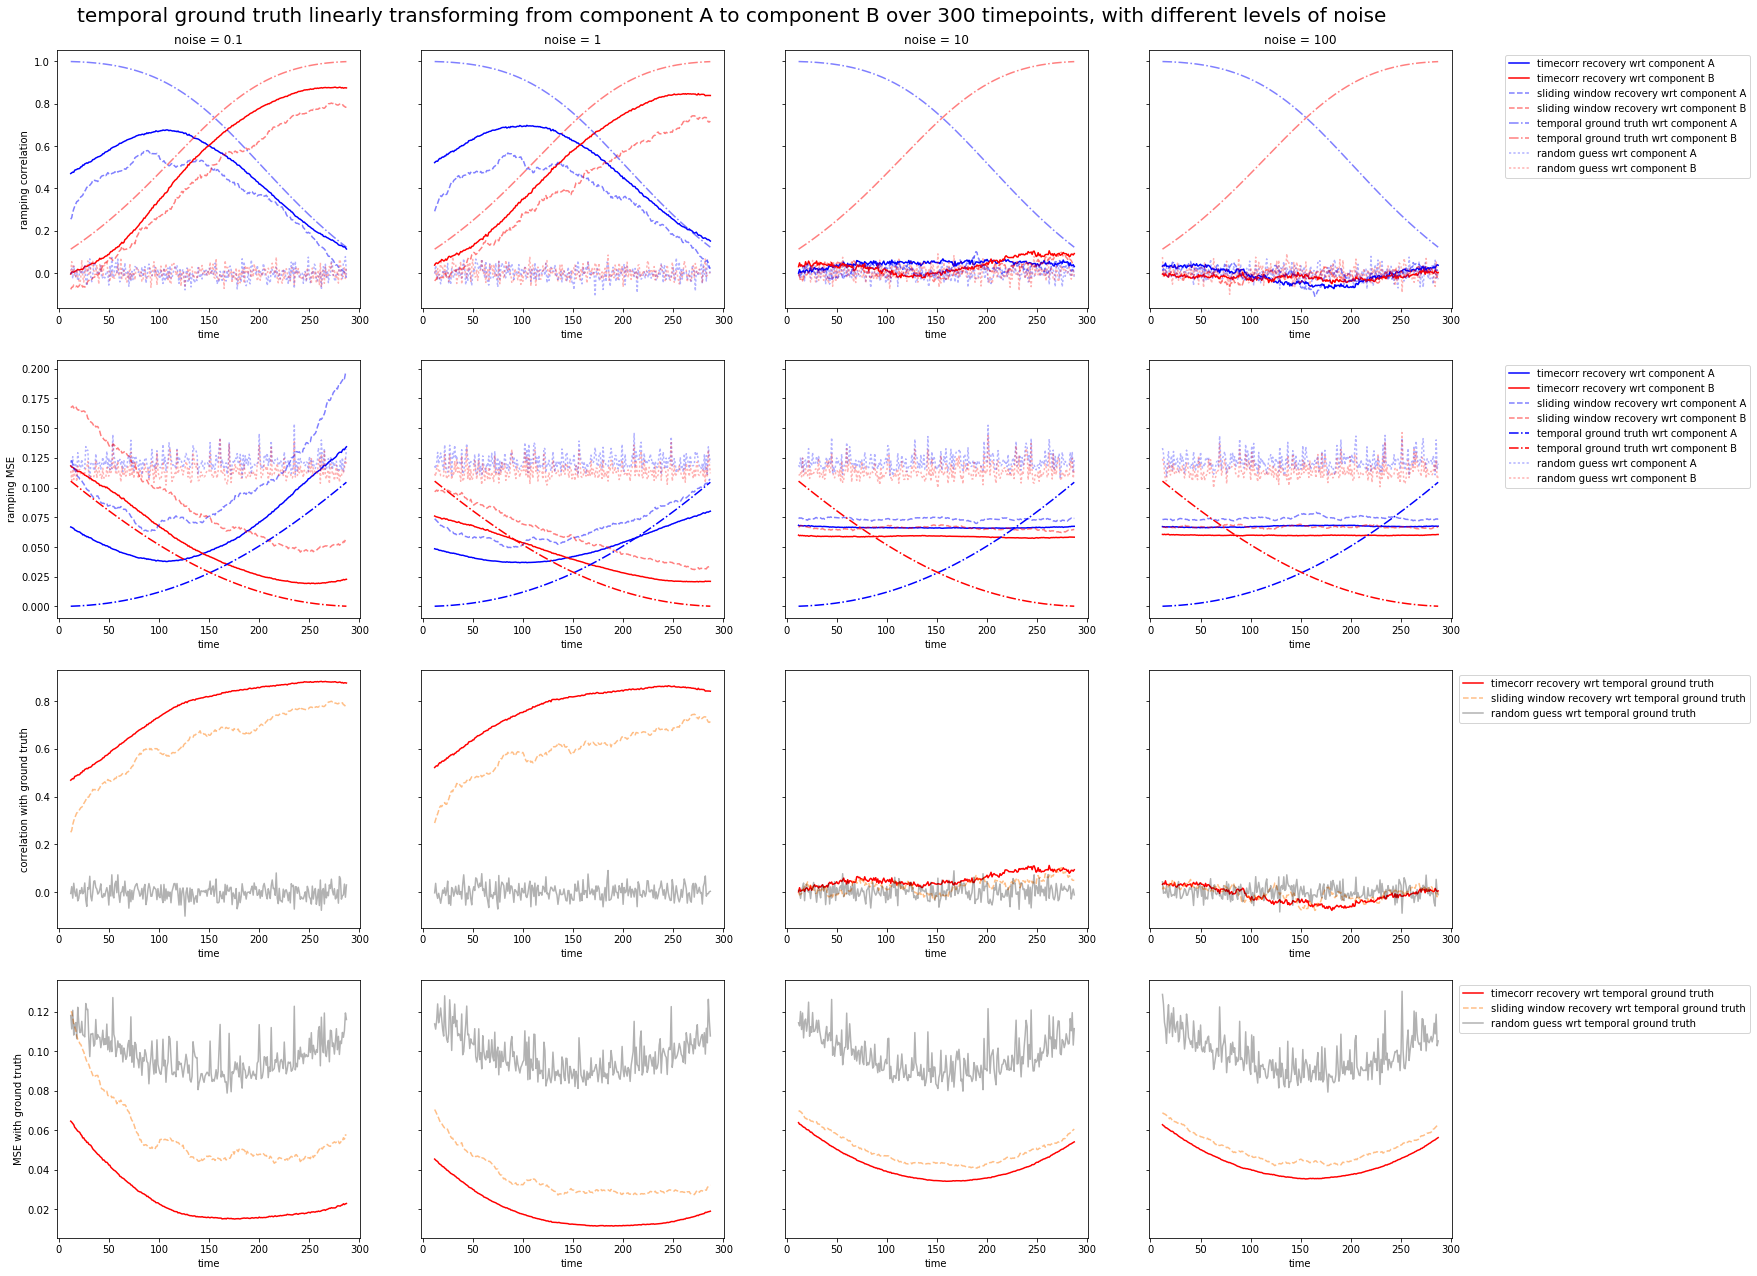
\includegraphics[width=1\textwidth]{../figures/ISFC/t300slide25var1000.png}
\label{fig:t300slide25var1000}
(a) In the first row, solid lines show the correlation between block correlations and TimeCorr solutions; dotted, sliding window solutions; dot-dashed, ground truth. (b) In the second row, solid lines show mean squared error(MSE) between block correlations and TimeCorr solutions; dotted, sliding window solutions; dot-dashed, ground truth. (c) In the third row, the solid line shows correlation between temporal ground truth and TimeCorr solutions; dotted, sliding window solutions; gray, random guess. (d) In the fourth row, the solid line shows MSE between temporal ground truth and TimeCorr solutions; dotted line, sliding window solutions; gray, random guess. (e) The columns represent recovery results from datasets with varying noise levels. (f) In the first two rows, the blue lines represent the relationship between recovered solution and the left terminal correlation; red line, right terminal correlation.
\end{figure}

The results show that TimeCorr is able to retrieve the stimulus-driven dynamic correlation structure with relatively high accuracy at low(0.1) to medium(1) noise levels, but fails to recover any meaningful information when the noise level is too high(10 and 100). These results highlight the difficulty of recovering stimulus-driven correlation structures when the subjects display weak cognitive response to the stimulus. However, when the stimuli is able to evoke reasonably strong cognitive response from the subject, TimeCorr can effectively recover the stimuli-driven dynamic correlation structures with relatively high accuracy.

In addition, due to the limited number of total time points in the dataset, we chose to use a sliding window setup with a window length of 25 time points. When comparing the correlation and MSE between their solutions and the temporal ground truths, the TimeCorr approach distinctly outperforms the sliding window method in every situation. Furthermore, as the amount of noise increases, the performance of the sliding window approach deteriorates more noticeably than that of the TimeCorr approach. These contrasts further consolidates TimeCorr as the superior choice for functional connectivity calculations.


\section{Decoding Analysis using TimeCorr ISFC}
Next, we evaluated how brain dynamics is represented by each level of high-order functional connectivity.

Elaborate on strictness of decoding analysis, which adds to the the credibility of its results.

Elaborate on steps used for this test.

Eleborate on how changing Gaussian variance resulted in a different distribution of decoding accuracy. Attribute difference to temporal resolution->different focus reveals different informaiton about the dynamics.

Compare with previous research results, Jeremy. Confirms timecorr is superior. Also PCA is more effective in preserving dynamic structure than HTFA, which in turn justifies it's usage in level up.

Elaborate on the temporal resolution potentially influencing the results, therefore conducted experiments with multiple setups. Some setups resulted in first level ISFC having higher decoding accuracy, which is very different from previous results.

Lower decoding accuracy, although the high order brain functional connectivity still contain information about the story times, there seems to have been a small amount of information loss in the transformation from voxel activations to node activations, leading to slightly lower classification accuracy.

\section{Multi-Level Mixture Analysis}
Although high-order functional connectivity returned low decoding accuracy, we were still curious whether the information would be useful. We hypothesize that the functional connectivity at each level represent non-overlapping sources of cognitively relevant information. Therefore a mixture model incorporating information from multiple levels could potentially result in higher decoding accuracy than any individual level.

Given a fMRI dataset for $S$ subjects, each possessing $T$ time points and $V$ voxels, to conduct Decoding Analysis:
\begin{enumerate}
\item Choose the desired number of levels of functional connectivities $L$ and the appropriate Gaussian variance for TimeCorr.
\item Use the TimeCorr Level Up method to obtain all level functional connectivites for each subject.
\item Randomly divide the subjects in to four equal groups $A_1$, $A_2$, $B_1$ and $B_2$.
\item For each group, use the Multi-Subject TimeCorr ISFC method to compute the inter-subject functional connectivity for each level
\item Compute correlation matrices for each level for A and B (i.e. for group A, correlate A1's features at each time point with A2's features at each time point; similarly for group B). This yields one correlation matrix for group A and another for group B, for each level (including level 0). So if we go up to level 10, this would be 11 correlation matrices for A and another 11 for B.
\item Fisher Z-transform all of the correlation matrices should be z-transformed (r2z). Let's call them $z_A0, z_A1, z_ A2, ..., z_B0, z_B1, z_B2, ..., z_B10$.
\item Use constrained optimization by linear approximation (COBYLA) on the group A correlation matrices to compute the weighting matrix w to be used for decoding-- i.e. $decoding_matrix_A = z2r(w[0]*z_A0 + w[1]*z_A1 + w[2]*z_A2 + ... + w[10]*z_A10)$. In other words, find the w that maximizes the decoding accuracy using $decoding_matrix_A$.
\item Now use the same z2r(<weighted z-transformed sum>) formula to compute decoding accuracy for group B
Save out w and the group B decoding accuracy
Collect the w and group B decoding accuracies across the 100 runs and summarize them in a figure
\end{enumerate}

Elaborate on training using half the dataset and testing on half the dataset, which caused the decoding accuracy to be a lot lower than when using the entire dataset.

Elaborate on weight distribution. Most information contained within first level ISFC. Consistent with high resolution result in single level decoding analysis, where first level functional connectivity achieved the highest decoding accuracy.

Elaborate on the temporal resolution potentially influencing the results, therefore conducted experiments with multiple setups. However, weight distribution remained the same with highest weight on first level functional connectivity. Which means that although sometime raw activations may result in higher decoding accuracy, most of the information on brain dynamics is actually contained in first level ISFC. This result was not available in previous researches because of the lack of freedom in choosing temporal resolution.

In addition, incorporating information from multiple levels resulted in significantly higher decoding accuracy than that of any individual level. This confirms our hypothesis that different levels contain non-overlapping information about brain dynamics and, although individual levels did not produce high classification accuracy, when used in unison can greatly enrich data complexity and increase decoding accuracy.

\begin{enumerate}
\item haha
\begin{enumerate}
\item Testing ISFC on block correlation dataset and comparison with sliding window results
\item Testing ISFC on ramp correlation dataset and comparison with sliding window results
\item Testing level up on multisubject ramping correlation dataset and comparison with sliding window results
\end{enumerate}
\item Results on the Pieman dataset
\begin{enumerate}
\item See Jeremy's paper for reference on order and structure of this section

\item Pieman Intact
\end{enumerate}
\item Results on Sherlock dataset
\item Results on Forrest dataset
\item Level-mixture analysis
\item Optimization and Benchmark results

\end{enumerate}


\section{Conclusion}
\begin{enumerate}
\item application in medicine for classification data enrichment
\end{enumerate}



\begin{enumerate}
\item \cite{jeremy2017} decoding analysis, ISFC
\item \cite{hasson2016} First time Inter-subject functional connectivity is introduced. opens new avenues for linking brain network dynamics to stimulus features and behavior.
\item \cite{khambhati2017} We describe recent efforts to model dynamic patterns of connectivity, dynamic patterns of activity, and patterns of activity atop connectivity. In the context of these models, we review important considerations in statistical testing, including parametric and non-parametric approaches. Finally, we offer thoughts on careful and accurate interpretation of dynamic graph architecture, and outline important future directions for method development.
\item \cite{davidson2016} we present a method to quantify individual differences in brain functional dynamics by applying hypergraph analysis, a method from dynamic network theory. age-related changes in brain function can be better understood by taking an integrative approach that incorporates information about the dynamics of functional interactions
\item \cite{peterson11} However, we find that observations of “dynamic” BOLD correlations during the resting state are largely explained by sampling variability. Beyond sampling variability, the largest part of observed “dynamics” during rest is attributable to head motion. An additional component of dynamic variability during rest is attributable to fluctuating sleep state. Thus, aside from the preceding explanatory factors, a single correlation structure—as opposed to a sequence of distinct correlation structures—may adequately describe the resting state as measured by BOLD fMRI. These results suggest that resting-state BOLD correlations do not primarily reflect moment-to-moment changes in cognitive content. Rather, resting-state BOLD correlations may predominantly reflect processes concerned with the maintenance of the long-term stability of the brain’s functional organization
\item \cite{peterson12} Machine Learning for classification. We also report a novel adaptation of SVM binary classification that, in addition to an overall accuracy rate for the SVM, provides a confidence measure for the accurate classification of each individual. Our results support the contention that multivariate methods can better capture the complexity of some brain disorders, and hold promise for predicting prognosis and treatment outcome for individuals with TS.
\item \cite{peterson17} Support vector regression enabled quantitative estimation of birth gestational age in single subjects using only term equivalent resting state-functional MRI data, indicating that the present approach is sensitive to the degree of disruption of brain development associatedwith pretermbirth (using gestational age as a surrogate for the extent of disruption). This suggests that support vector regression may provide a means for predicting neurodevelopmental outcome in individual infants.
\item \cite{olaf2005} First time research is conducted in brain functional connectivity, it's significance is revealed.
\item \cite{hasson2012} Here we show that temporal patterns of neural activity contain information that can discriminate different stimuli, even within brain regions that show no net activation to that stimulus class. Furthermore, we find that in many brain regions, responses to natural stimuli are highly context dependent. In such cases, prototypical event-related responses do not even exist for individual stimuli, so that averaging responses to the same stimulus within different contexts may worsen the effective signal-to-noise. As a result, analysis of the temporal structures of single events can re
\item \cite{enrico2011} Sliding window, instantaneous phase synchronization to increase temporal resolution, Dynamic Functional Connectivity
\item \cite{Greene01} The long-standing rationalist tradition in moral psychology emphasizes the role of reason in moral judgment. A more recent trend places increased emphasis on emotion. Although both reason and emotion are likely to play important roles in moral judgment, relatively little is known about their neural correlates, the nature of their interaction, and the factors that modulate their respective behavioral influences in the context of moral judgment. In two functional magnetic resonance imaging (fMRI) studies using moral dilemmas as probes, we apply the methods of cognitive neuroscience to the study of moral judgment. We argue that moral dilemmas vary systematically in the extent to which they engage emotional processing and that these variations in emotional engagement influence moral judgment.
\item \cite{Logothetis01} Functional magnetic resonance imaging (fMRI) is widely used to study the operational organization of the human brain, but the exact relationship between the measured fMRI signal and the underlying neural activity is unclear. These findings suggest that the BOLD contrast mechanism reflects the input and intracortical processing of a given area rather than its spiking output.
\item \cite{hasson2005} AUDIO The predicted fMRI signals derived from single units and the measured fMRI signals from auditory cortex showed a highly significant correlation (r 0 0.75, P G 10j47). Thus, fMRI signals can provide a reliable measure of the firing rate of human cortical neurons.
\item \cite{hasson2004} VIDEO The results reveal a surprising tendency of individual brains to “tick collectively” during natural vision. The intersubject synchronization consisted of a widespread cortical activation pattern correlated with emotionally arousing scenes and regionally selective components. The characteristics of these activations were revealed with the use of an open-ended “reverse-correlation” approach, which inverts the conventional analysis by letting the brain signals themselves “pick up” the optimal stimuli for each specialized cortical area.
\item \cite{peterson9} various denoising methods
\item \cite{peterson19} We suggest that, in the place of a single localized error mechanism, these findings point to a large-scale set of error-related regions across multiple systems that likely subserve different functions.
\item \cite{peterson20} In 2011, three groups reported that small headmovements produced spurious but structured noise in brain scans, causing distance-dependent changes in signal correlations. This finding has prompted both methods development and the re-examination of prior findings with more stringentmotion correction
\end{enumerate}
\begin{thebibliography}{1}
\bibitem{jeremy2017} Jeremy Manning, Xia Zhu, Theodore Willke, Rajesh Ranganath, Kimberly Stachenfeld, Uri Hasson, David M Blei, Kenneth A Norman. A probabilistic approach to discovering dynamic full-brain functional connectivity patterns. \textit{bioRxiv} 106690, 2017
\bibitem{elena2012} Elena A. Allen, Eswar Damaraju, Sergey M. Plis, Erik B. Erhardt, Tom Eichele and Vince D. Calhoun. Tracking Whole-Brain Connectivity Dynamics in the Resting State. \textit{Cerebral Cortex} March 2014;24:663–676
\bibitem{enrico2011} Enrico Glerean, Juha Salmi, Juha M. Lahnakoski, Iiro P. Jaaskelainen, and Mikko Sams. Functional Magnetic Resonance Imaging Phase Synchronization as a Measure of Dynamic Functional Connectivity. \textit{BRAIN CONNECTIVITY} Volume 2, Number 2, 2012
\bibitem{olaf2005} Olaf Sporns, Giulio Tononi, Rolf Kotter. The Human Connectome: A Structural Description of the Human Brain. \textit{PLOS Computational Biology} September 2005
\bibitem{hasson2016} Erez Simony, Christopher J. Honey, Janice Chen, Olga Lositsky, Yaara Yeshurun, Ami Wiesel and Uri Hasson. Dynamic reconfiguration of the default mode network during narrative comprehension. \textit{nature communications} July, 2016
\bibitem{davidson2016} Elizabeth N. Davison, Benjamin O. Turner, Kimberly J. Schlesinger, Michael B. Miller, Scott T. Grafton, Danielle S. Bassett, Jean M. Carlson. Individual Differences in Dynamic Functional Brain Connectivity Across the Human Lifespan. \textit{arXiv}:1606.09545v1
\bibitem{tang2017} Evelyn Tang and Danielle S. Bassett. Control of Dynamics in Brain Networks. \textit{arXiv}:1701.01531v2
\bibitem{khambhati2017} Ankit N. Khambhati, Ann E. Sizemore, Richard F. Betzel, and Danielle S. Bassett. Modelling and Interpreting Network Dynamics. \textit{bioRxiv} Apr. 4, 2017.
\bibitem{hasson2009} Uri Hasson, Rafael Malach and David J. Heeger. Reliability of cortical activity during natural stimulation. \textit{Cell Press} December 2009
\bibitem{hasson2005} Roy Mukamel, Hagar Gelbard, Amos Arieli, Uri Hasson, Itzhak Fried and Rafael Malach. Coupling Between Neuronal Firing, Field Potentials, and fMRI in Human Auditory Cortex. \textit{SCIENCE} VOL 309 5 AUGUST 2005
\bibitem{hasson2004} Uri Hasson, Yuval Nir, Ifat Levy, Galit Fuhrmann and Rafael Malach. Intersubject Synchronization of Cortical Activity During Natural Vision. \textit{SCIENCE} 12 MARCH 2004 VOL 303.
\bibitem{hasson2012} Aya Ben-Yakova, Christopher J. Honey, Yulia Lerner and Uri Hasson. Loss of reliable temporal structure in event-related averaging of naturalistic stimuli. \textit{NeuroImage} 63 (2012) 501–506
\bibitem{zubeidi2014} Duha Al-Zubeidi, Mathula Thangarajh, PhDb, Sheel Pathak, Chunyu Cai, Bradley L. Schlaggar, Gregory A. Storch, Dorothy K. Grange and Michael E. Watson Jr.
\bibitem{peterson9} Gregory C. Burgess, Sridhar Kandala, Dan Nolan, Timothy O. Laumann, Jonathan D. Power, Babatunde Adeyemo, Michael P. Harms, Steven E. Petersen, and Deanna M. Barch. Evaluation of Denoising Strategies to Address Motion-Correlated Artifacts in Resting-State Functional Magnetic Resonance Imaging Data from the Human Connectome Project. \textit{BRAIN CONNECTIVITY} Volume 6, Number 9, 2016
\bibitem{peterson10} Evan M. Gordon, Timothy O. Laumann, Babatunde Adeyemo, Adrian W. Gilmore, Steven M. Nelson, Nico U.F. Dosenbach, Steven E. Petersen. Individual-specific features of brain systems identified with resting state functional correlations. \textit{NeuroImage} 146 (2017) 918–939
\bibitem{peterson11} Timothy O. Laumann, Abraham Z. Snyder, Anish Mitra, Evan M. Gordon, Caterina Gratton, Babatunde Adeyemo, Adrian W. Gilmore, Steven M. Nelson, Jeff J. Berg5, Deanna J. Greene, John E. McCarthy, Enzo Tagliazucchi, Helmut Laufs, Bradley L. Schlaggar, Nico U. F. Dosenbach, and Steven E. Petersen. On the Stability of BOLD fMRI Correlations
\bibitem{peterson12} Deanna J. Greene, Jessica A. Church, Nico U.F. Dosenbach, Ashley N. Nielsen, Babatunde Adeyemo, Binyam Nardos, Steven E. Petersen, Kevin J. Black and Bradley L. Schlaggar. Multivariate pattern classification of pediatric Tourette syndrome using functional connectivity MRI. \textit{Developmental Science} 19:4 (2016), pp 581–598
\bibitem{peterson17} Christopher D. Smyser, Nico U.F. Dosenbach, TaraA. Smyser, AbrahamZ. Snyder, Cynthia E. Rogers, Terrie E. Inder, Bradley L. Schlaggar and Jeffrey J. Neil. Prediction of brain maturity in infants using machine-learning algorithms. \textit{NeuroImage} 136 (2016) 1–9
\bibitem{peterson19} Maital Neta, XFrancis M. Miezin, Steven M. Nelson, Joseph W. Dubis, Nico U.F. Dosenbach, Bradley L. Schlaggar and Steven E. Petersen. Spatial and Temporal Characteristics of Error-Related Activity in the Human Brain. The Journal of Neuroscience, January 7, 2015
\bibitem{peterson20} Jonathan D. Power, Bradley L. Schlaggar, and Steven E. Petersen. Recent progress and outstanding issues in motion correction in resting state fMRI. \textit{NeuroImage} 105 (2015) 536–551
\bibitem{Logothetis01} Nikos K. Logothetis, Jon Pauls, Mark Augath, Torsten Trinath and Axel Oeltermann. Neurophysiological investigation of the basis of the fMRI signal. \textit{Nature} 412, 150-157 (12 July 2001)
\bibitem{Greene01}Joshua D. Greene, R. Brian Sommerville, Leigh E. Nystrom, John M. Darley and Jonathan D. Cohen. An fMRI Investigation of Emotional Engagement in Moral Judgment. \textit{Science}  14 Sep 2001: Vol. 293, Issue 5537
\bibitem{Friston99} K.J. Friston, A. Holmes, C.J. Price, C. Buchela and K.J. Worsley. Multisubject fMRI Studies and Conjunction Analyses. \textit{NeuroImage} Volume 10, Issue 4, October 1999
\bibitem{Friston98} K.J. Friston, P. Fletcher, O. Josephs, A. Holmes, M.D. Rugg and R. Turner. Event-Related fMRI: Characterizing Differential Responses. \textit{NeuroImage} Volume 7, Issue 1, January 1998
\bibitem{Ogawa90} S. Ogawa, T. M. Lee, A. R. Kay, and D. W. Tank. Brain magnetic resonance imaging with contrast dependent on blood oxygenation. \textit{PNAS} December 1, 1990
\bibitem{Norman06} Kenneth A. Norman, Sean M. Polyn, Greg J. Detre and James V. Haxby. Beyond mind-reading: multi-voxel pattern analysis of fMRI data. \textit{Trends in Cognitive Science} (2006)
\bibitem{Turke13} Nicholas B. Turk-Browne. Functional Interactions as Big Data in the Human Brain. \textit{SCIENCE} (342) November 1st, 2013.
\bibitem{Rubinov2010} M. Rubinov and O. Sporns. Complex network measures of brain connectivity: uses and interpretations. \textit{NeuroImage}, 52:1059-1069, 2010.
\bibitem{Betzel2017} R. E. Betzel, J. D. Medaglia, L. Papadopoulos, G. Baum, R. Gur, R. Gur, D. Roalf, T. D. Satterthwaite, and D. S. Bassett. The modular organization of human anatomical brain networks: accounting for the cost of wiring. \textit{Network Neuroscience}, page Advance online publication. doi:10.1162/netn.a.00002., 2017.
\bibitem{Craddock2012} R. C. Craddock, G. A. James, I. P E Holtzheimer, X. P. Hu, and H. S. Mayberg. A while brain fmri atlas generated via spatially constrained spectral clustering. \textit{Human Brain Mapping}, 33(8):1914-1928, 2012.
\bibitem{Yeo2011} B. T. T. Yeo, F. M. Krienen, J. Sepulcre, M. R. Sabuncu, D. Lashkari, M. Hollinshead, J. L. Roffman, J. W. Smoller, L. Zollei, J. R. Polimieni, B. Fischl, H. Liu, and R. L. Buckner. The organization of the human cerebral cortex estimated by intrinsic functional connectivity. \textit{Journal of Neurophsiology}, 106(3):1125-1165, 2011.
\end{thebibliography}
\end{document}
